\documentclass[12pt, a4j]{jsarticle}
\usepackage{additional}

\title{メディア情報学実験 最終レポート}
\author{1710730 須藤敬仁}
\date{}

\begin{document}
  \maketitle
  \section{実験方法}
    表\ref{table:pv}の20本のPVを視聴し, 表\ref{table:question}に示した21項目のアンケートを実施する.  
    %
    アンケートにはその質問内容に対して1(まったくそう思わない)から5(非常にそう思う)の5段階評価で答える.  
    各PVにおいてアンケートを実施した結果を集計し, そのデータに対して多変量解析を適用する.  

    \begin{table}[htb]
      \begin{minipage}[t]{.50\textwidth}
        \begin{center}
          \caption{実験対象PV}
          \scalebox{0.7}{
          \begin{tabular}{|c|c|c|} \hline 
            ID & 楽曲名 & 歌手名 \\ \hline \hline
            PV01 & ボーイフレンド & aiko  \\ \hline
            PV02 & 波乗りジョニー & 桑田圭祐  \\ \hline
            PV03 & 天体観測 & bump of chicken \\ \hline 
            PV04 & HANABI & Mr Children \\ \hline 
            PV05 & ただ会いたくて & EXILE \\ \hline
            PV06 & また君に恋してる & 坂本冬美 \\ \hline 
            PV07 & 夏色 & ゆず \\ \hline 
            PV08 & Endless Sorrow & 浜崎あゆみ \\ \hline 
            PV09 & 真夜中は純潔 & 椎名林檎 \\ \hline 
            PV10 & 桜坂 & 福山雅治 \\ \hline 
            PV11 & sailing day  & bump of chicken \\ \hline 
            PV12 & Everything & Misia \\ \hline 
            PV13 & Drivers High & L'Arc-en-Ciel \\ \hline 
            PV14 & Can You Keep A Secret? & 宇多田ヒカル \\ \hline 
            PV15 & 白い恋人達 & 桑田圭祐 \\ \hline 
            PV16 & きよしのズンドコ節 & 氷川きよし \\ \hline 
            PV17 & GIFT & Mr Children \\ \hline 
            PV18 & Real World & EXILE \\ \hline 
            PV19 & 逢いたくていま & Misia \\ \hline 
            PV20 & M & 浜崎あゆみ \\ \hline 
          \end{tabular}
          }
        \end{center}
        \label{table:pv}  
      \end{minipage}
      %
      \hfill
      %
      \begin{minipage}[t]{.45\textwidth}
        \begin{center}
          \caption{アンケート内容}
          \scalebox{0.7}{
          \begin{tabular}{|c|c|c|} \hline 
            質問番号 & カテゴリ & 質問内容 \\ \hline \hline
            Q1 &         & 洗練されている\\ \cline{1-1} \cline{3-3}
            Q2 & 雰囲気が & 親しみやすい  \\ \cline{1-1} \cline{3-3}
            Q3 &         & 好きだ        \\ \hline
            Q4 &         & 洗練されている\\ \cline{1-1} \cline{3-3}
            Q5 & アーティストが & 親しみやすい  \\ \cline{1-1} \cline{3-3}
            Q6 &         & 好きだ        \\ \hline
            Q7 &         & 洗練されている\\ \cline{1-1} \cline{3-3}
            Q8 & 映像が   & 見やすい  \\ \cline{1-1} \cline{3-3}
            Q9 &         & 迫力がある  \\ \cline{1-1} \cline{3-3}
            Q10 &         & 好きだ        \\ \hline
            Q11&         & 洗練されている\\ \cline{1-1} \cline{3-3}
            Q12 & メロディが   & 聞きやすい  \\ \cline{1-1} \cline{3-3}
            Q13 &         & 迫力がある  \\ \cline{1-1} \cline{3-3}
            Q14 &         & 好きだ        \\ \hline
            Q15 &         & 洗練されている\\ \cline{1-1} \cline{3-3}
            Q16 & 歌詞が & 分かりやすい  \\ \cline{1-1} \cline{3-3}
            Q17 &         & 好きだ        \\ \hline
            Q18 &         & 印象に残る \\ \cline{1-1} \cline{3-3}
            Q19 & 全体として & 楽曲が欲しくなる  \\ \cline{1-1} \cline{3-3}
            Q20 &         & 好きだ        \\ \hline
            Q21 & この曲を & 知っている \\ \hline
          \end{tabular}
          }
        \end{center}
        \label{table:question}   
      \end{minipage}
    \end{table}

  \section{a-sumの分析}
    a-sumは各PVに対するアンケート結果をPVごとに合計値を算出したデータである. 
    この分析では目的変数であるQ20と1か5かほぼ2値の値を取るQ21を除外して分析を行う.  
    
    \subsection{積み上げ棒グラフ}
      a-sumの積み上げ棒グラフを図\ref{fig:asum_bar}に示す. 表\ref{table:question}
      の質問からわかる通り, どの項目も数値が高いほど高評価になるような質問である. 
      つまり, 合計値が大きいほど対象PVの評価が高い傾向にある. 図\ref{fig:asum_bar}から, 
      PV01, PV08は比較的評価が低く, PV03, PV07, PV15は評価が高いことが観察できる. 

      % figure : a-sum/bar.bmp 
      \begin{figure}[htb]
        \centering
        \includegraphics[width=7cm]{../2nd/a-sum/bar.bmp}
        \caption{a-sumの積み上げ棒グラフ}
        \label{fig:asum_bar}
      \end{figure}

    \subsection{不偏分散値・標準偏差}
      各質問に対しての不偏分散値及び標準偏差を表\ref{table:asum_std}に示す. 
      標準偏差が大きいほどデータのばらつきがあるので, 区分を持たせるときに有用なデータであると考えられる. 
      表\ref{table:asum_std}からQ2, Q7, Q9, Q16などが標準偏差が大きいことがわかる. 

      \begin{table}
        \centering
        \caption{不偏分散値・標準偏差(a-sum)}
        \scalebox{0.7}{
        \begin{tabular}{|c|c|c|} \hline 
          質問 & 不偏分散値 & 標準偏差 \\ \hline \hline 
          Q1 & 45262.15 & 212.75 \\ \hline 
          Q2 & 70052.67 & 264.67 \\ \hline 
          Q3 & 27458.47 & 165.71 \\ \hline 
          Q4 & 20320.74 & 142.55 \\ \hline 
          Q5 & 62576.87 & 250.13 \\ \hline 
          Q6 & 37687.54 & 194.13 \\ \hline 
          Q7 & 78300.16 & 279.82 \\ \hline 
          Q8 & 38201.67 & 195.45 \\ \hline 
          Q9 & 146846.2 & 383.21 \\ \hline 
          Q10 & 30689.54 & 175.18 \\ \hline 
          Q11 & 20960.05 & 144.78 \\ \hline 
          Q12 & 39887.10 & 199.72 \\ \hline 
          Q13 & 47275.84 & 217.43 \\ \hline 
          Q14 & 37493.64 & 193.63 \\ \hline 
          Q15 & 28118.26 & 167.69 \\ \hline 
          Q16 & 77776.77 & 278.88 \\ \hline 
          Q17 & 36403.11 & 190.80 \\ \hline 
          Q18 & 29305.91 & 171.19 \\ \hline 
          Q19 & 45944.34 & 214.35 \\ \hline 
        \end{tabular}
        }
        \label{table:asum_std}
      \end{table}

    \subsection{主成分分析}
      データa-sumに対して主成分分析を行った. 各主成分の固有値と累積寄与率を
      示したグラフを図\ref{fig:asum_eval}に示す. 固有値1.0以上及び累積寄与率
      80\%を基準として, 図\ref{fig:asum_eval}から主成分の数を3つとする. この
      3つの主成分を基にa-sumに対して分析を行う. 

      \begin{figure}[htb]
        \centering
        \includegraphics[width=7cm]{../2nd/a-sum/scree.bmp}
        \caption{各主成分の固有値と累積寄与率(a-sum)}
        \label{fig:asum_eval}
      \end{figure}

      \subsubsection{主成分負荷量と名前付け}
      3つの主成分について主成分負荷量を表\ref{table:asum_fl}に示す. 
      表\ref{table:asum_fl}からPC1に対して, 質問Q3, Q6, Q11, Q14, Q15, Q17, Q19が
      大きな影響を与えている. これらの主成分負荷量は負の値を取っているため, 
      表\ref{table:question}からPC1には「好みでない曲」という名前をつけた.  

      次にPC2に対しては, 質問Q1, Q4, Q7, Q9が大きな影響を与えている. これらは
      正の値の主成分負荷量を取っているため, PC2には「見た目の洗練さ」という名前を
      つけた.  

      最後にPC3に対しては, 質問Q1, Q4, Q15, Q16が負の主成分負荷量を取り, 質問Q9, Q13
      は正の主成分負荷量を取っている. これらがPC3に影響を与えているため, PC3には
      「他を犠牲にした迫力」という名前をつけた. 

      \begin{table}
        \centering
        \caption{a-sumの3主成分に対する主成分負荷量}
        \scalebox{0.7}{
        \begin{tabular}{|c|c|c|c|} \hline
          質問 & PC1 & PC2 & PC3 \\ \hline \hline 
          Q1 & -0.147 & 0.851 & -0.463 \\ \hline 
          Q2 & -0.693 & -0.47 & 0.363 \\ \hline 
          Q3 & -0.871 & 0.311 & 0.334 \\ \hline 
          Q4 & -0.337 & 0.718 & -0.495 \\ \hline 
          Q5 & -0.683 & -0.507 & 0.306 \\ \hline 
          Q6 & -0.852 & 0.0533 & 0.351 \\ \hline 
          Q7 & 0.0512 & 0.916 & -0.234 \\ \hline 
          Q8 & -0.566 & 0.25 & -0.367 \\ \hline 
          Q9 & 0.306 & 0.692 & 0.575 \\ \hline 
          Q10 & -0.49 & 0.715 & 0.397 \\ \hline 
          Q11 & -0.865 & 0.193 & -0.384 \\ \hline 
          Q12 & -0.767 & -0.472 & -0.336 \\ \hline 
          Q13 & -0.0945 & 0.65 & 0.453 \\ \hline 
          Q14 & -0.946 & -0.0236 & 0.128 \\ \hline 
          Q15 & -0.852 & 0.152 & -0.409 \\ \hline 
          Q16 & -0.61 & -0.447 & -0.502 \\ \hline 
          Q17 & -0.947 & -0.121 & 0.0318 \\ \hline 
          Q18 & -0.689 & 0.0059 & 0.298 \\ \hline 
          Q19 & -0.901 & 0.183 & 0.23 \\ \hline 
        \end{tabular}
        }
        \label{table:asum_fl}
      \end{table}

      \subsubsection{散布図}
      各主成分を軸とした散布図を図\ref{fig:asum_sc}に示す. 図\ref{fig:asum_sc12}及び
      \ref{fig:asum_sc13}からPV3, PV7, PV15の曲が好まれる傾向にあることが分かる. これは
      積み上げ棒グラフによる分析を裏付けるような結果となっている. つまり, 第一主成分である
      ことからPVが好きかどうか(目的変数)に対して曲が好みかどうかの影響が大きく, それらの
      関係性が積み上げ棒グラフと散布図から見て取れているということがわかる.  

      \begin{figure}
        \begin{center}
          \subfigure[PC1とPC2]{
            \includegraphics[width=4cm]{../2nd/a-sum/2d-scatter_p1xp2.bmp}
            \label{fig:asum_sc12}
          }
          %
          \hfill
          %
          \subfigure[PC1とPC3]{
            \includegraphics[width=4cm]{../2nd/a-sum/2d-scatter_p1xp3.bmp}
            \label{fig:asum_sc13}
          }
          % 
          \hfill 
          %
          \subfigure[PC2とPC3]{
            \includegraphics[width=4cm]{../2nd/a-sum/2d-scatter_p2xp3.bmp}
            \label{fig:asum_sc23}
          }
        \end{center}
        \vspace{-0.5cm}
        \caption{各主成分軸同士での散布図}
        \label{fig:asum_sc}
      \end{figure}
    \subsection{重回帰分析}
      Q20を目的変数, 選択した主成分PC1からPC3を説明変数として重回帰分析を行った. 
      分析の結果, 決定係数は$R^2$=.97であり, 0.1\%水準で有意であった(F(3,16)=154.3, p $<$ .001). 
      求めた重回帰式を式\ref{eq:asum}, パス図を図\ref{fig:asum_path}に示す. 

      \begin{equation}
        Q20 = (-62.55) * PC1 + 10.75 * PC2 + (-28.55) * PC3 + 1964.75
        \label{eq:asum}
      \end{equation}

      \begin{figure}
        \centering
        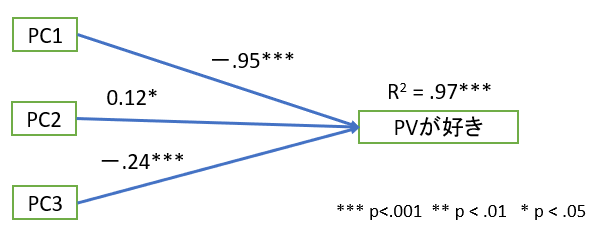
\includegraphics[width=8cm]{../2nd/a-sum/path.png}
        \caption{パス図(a-sum)}
        \label{fig:asum_path}
      \end{figure}
    \subsection{クラスタ分析}
      アンケート結果全項目についてウォード法によるクラスタ分析を行った
      結果を図\ref{fig:asum_dendrogram}のデンドログラムに示す. 
      図\ref{fig:asum_dendrogram}からQ21が極端な値を取りやすい質問であり, 
      ほかの問題と傾向が違う独自クラスタであることが分かる. また, 低い
      階層で分岐が起こっている変数同士は質問内容や質問カテゴリが同一であるもの
      がほとんどである. また, 主成分分析で選択した主成分に強く影響与える変数同士が
      同クラスタに分類されていることから, クラスタ分析から主成分分析の有効性を判断できる. 

      \begin{figure}[htb]
        \centering
        \includegraphics[width=8cm]{../2nd/a-sum/cluster.bmp}
        \caption{デンドログラム(a-sum)}
        \label{fig:asum_dendrogram}
      \end{figure}
  \section{担当PV(PV06)の分析}
    \subsection{分析PV : また君に恋してる / 坂本冬美}
      この楽曲のジャンルはフォークソングに分類される. 元々は2名の男性ユニット「ビリー・バンバン」
      によるオリジナル曲で, それをカバーしたものである. 楽曲とPVともに落ち着いていて大人びた
      印象がある楽曲であり, この雰囲気が気に入るかどうかが「PVが好き」かどうかの大きな
      要因ではないかと仮説を立て分析を行った. 
    \subsection{主成分分析}
      PV06に対して説明変数であるQ20, 特殊な質問であるQ21を除いて主成分分析を行った. 
      各主成分の固有値と累積寄与率を示したグラフを図\ref{fig:pv06_eval}に示す. 
      図\ref{fig:pv06_eval}から固有値1.0以上, 累積寄与率80\%を基準として主成分
      の選定を行った結果, PC1からPC5までの主成分で分析を行った. 

      \begin{figure}[htb]
        \centering
          \includegraphics[width=7cm]{../2nd/pv06/scree.bmp}
        \caption{各主成分の固有値と累積寄与率(PV06)}
        \label{fig:pv06_eval}
      \end{figure}

    \subsection{重回帰分析}
      Q20を目的変数, 選択した主成分PC1からPC5を説明変数として重回帰分析を行った. 
      分析の結果, 決定係数は$R^2$=.63であり, 0.1\%水準で有意であった(F(5,557)=194.2, 
      p $<$ .001). パス図を図\ref{fig:pv06_path1}に示す. 図\ref{fig:pv06_path1}
      からPC4に対応する標準化偏回帰係数が小さい為, 分析には不要な変数として判断し, 
      PC4を説明変数から除いた状態で再度重回帰分析を行った. 
      分析の結果, 決定係数は$R^2$=.63であり, 0.1\%水準で有意であった(F(4,578)=242.6,
      p $<$ .001). 
      最終的なパス図を図\ref{fig:pv06_path2}, 重回帰式を式\ref{eq:pv06}に示す. 
      図\ref{fig:pv06_path2}から全ての主成分において0.1\%で統計的に有意であること
      わかる. また, 最も標準化偏回帰係数が大きいPC1が目的変数(PVが好き)に強い
      影響を与えていることがわかる. PC1の偏回帰係数は負である為, PC1が増大する
      程に目的変数(PVが好き)が減少する関係がある. 

      \begin{eqnarray}
        Q20 &=& (-0.294) * PC1 + (-0.149) * PC2 \nonumber \\
            & & +\ 0.174 * PC3 + 0.154 * PC5 + 3.13
        \label{eq:pv06}
      \end{eqnarray}
      
      \begin{figure}[htb]
        \centering
        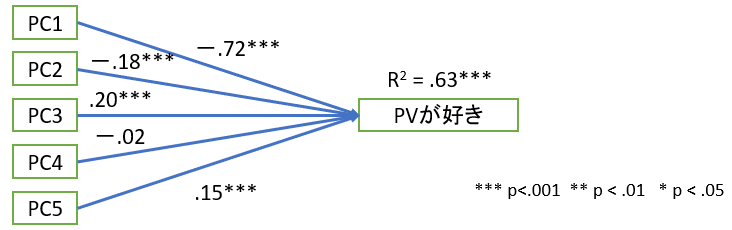
\includegraphics[width=8cm]{../2nd/pv06/path1.png}
        \caption{主成分PC1からPC5を利用したパス図}
        \label{fig:pv06_path1}
      \end{figure}

      \begin{figure}[htb]
        \centering
        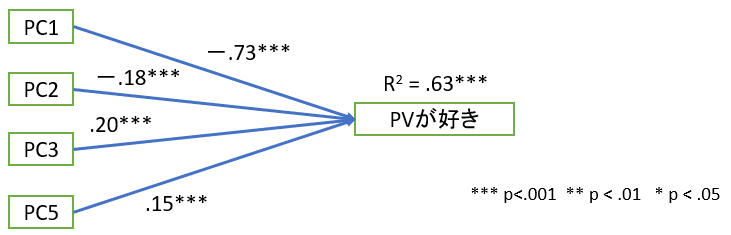
\includegraphics[width=8cm]{../2nd/pv06/path2.png}
        \caption{不要な主成分PC4を除いたパス図}
        \label{fig:pv06_path2}
      \end{figure}
    \subsection{各主成分の考察}
      重回帰分析でQ20の説明変数とした主成分PC1, PC2, PC3, PC5について
      主成分負荷量から考察を行う. 主成分負荷量を表\ref{fig:pv06_fs}に示す. 

      \begin{table}
        \centering
        \caption{各主成分の主成分負荷量(PV06)}
        \scalebox{0.7}{
        \begin{tabular}{|c|c|c|c|c|} \hline
          質問 & PC1 & PC2 & PC3 & PC5 \\ \hline \hline 
          Q1 & -0.58 & 0.0991 & -0.488 & 0.211 \\ \hline
          Q2 & -0.511 & -0.237 & -0.258 & -0.0743 \\ \hline
          Q3 & -0.752 & -0.299 & -0.109 & 0.169 \\ \hline
          Q4 & -0.619 & 0.216 & -0.205 & 0.258 \\ \hline
          Q5 & -0.487 & -0.271 & -0.113 & -0.0303 \\ \hline
          Q6 & -0.729 & -0.244 & 0.0864 & 0.224 \\ \hline
          Q7 & -0.514 & -0.111 & -0.52 & -0.0715 \\ \hline
          Q8 & -0.437 & 0.252 & -0.349 & -0.519 \\ \hline
          Q9 & -0.328 & -0.55 & 0.153 & -0.45 \\ \hline
          Q10 & -0.595 & -0.405 & -0.253 & -0.205 \\ \hline
          Q11 & -0.657 & 0.399 & 0.0929 & 0.0149 \\ \hline
          Q12 & -0.618 & 0.484 & 0.07 & -0.171 \\ \hline
          Q13 & -0.475 & -0.0796 & 0.534 & -0.308 \\ \hline
          Q14 & -0.761 & -0.00427 & 0.301 & 0.124 \\ \hline
          Q15 & -0.63 & 0.365 & 0.0124 & 0.145 \\ \hline
          Q16 & -0.534 & 0.46 & 0.0447 & -0.305 \\ \hline
          Q17 & -0.727 & -0.0154 & 0.238 & 0.0986 \\ \hline
          Q18 & -0.501 & 0.055 & 0.334 & -0.0133 \\ \hline
          Q19 & -0.697 & -0.257 & 0.254 & 0.24 \\ \hline
        \end{tabular}
        }
        \label{fig:pv06_fs}
      \end{table}
      
      \subsubsection{PC1}
        表\ref{fig:pv06_fs}をみると, 影響が大きい質問にはQ3, Q6, Q14, Q17
        が挙げられる. これらの質問はそれぞれ映像以外に関して好きかどうかを問う
        質問となっている. 映像に関しての質問(Q7, Q8, Q9, Q10)の主成分負荷量は
        比較的小さい値を取っているので, PC1は映像より楽曲が好きかどうかを
        測る軸であると考えられる. また, これら主成分負荷量の値は負の符号を取っている
        ので, PC1には「楽曲の嫌い度」と名前を付けた. \ref{fig:pv06_path2}に
        も示した通り, 確かにPC1の値が増大すれば目的変数(PVが好きだ)の値が減少する
        と言えそうである. 
      
      \subsubsection{PC2}
        表\ref{fig:pv06_fs}からPC2に主に影響している質問はQ9, Q10, Q12, Q16である. 
        符号に注意してPC2に影響している質問内容を考えるとそれぞれ, Q9「映像に迫力がない」,
        Q10「映像が嫌い」, Q12「メロディが聞きやすい」, Q16「歌詞が分かりやすい」となる. 
        よって, PC2には「PVの落ち着き具合」という名前を付けた. 

      \subsubsection{PC3}
        表\ref{fig:pv06_fs}からPC3に主に影響している質問はQ1, Q7, Q13である. 
        符号を考慮した質問内容は, Q1「雰囲気が洗練されていない」, Q7「映像が洗練されていない」, 
        Q13「メロディに迫力がある」となる. これらから, PC3には「PVよりも迫力のあるメロディ」
        と名前を付けた. 
      
      \subsubsection{PC5}
        表\ref{fig:pv06_fs}からPC5に主に影響している質問はQ8, Q9である. 
        符号を考慮した質問内容は, Q8「映像が見にくい」, Q9「映像に迫力がない」となる. 
        これらから, PC5には「目立ちすぎないPV」と名前を付けた. 

      \subsubsection{各主成分の総括}
        各主成分の名前についてまとめると表\ref{fig:names}となる. これらから
        目的変数を説明する要因を一言でまとめると「PVが楽曲を引き立てているか」
        と結論づけた. 

        \begin{table}
          \centering
          \caption{各主成分の名前(PV06)}
          \begin{tabular}{|c|c|c|} \hline 
            主成分 & 符号 & 名前 \\ \hline \hline 
            PC1 & 負 & 楽曲の嫌い度 \\ \hline
            PC2 & 負 & PVの落ち着き具合 \\ \hline
            PC3 & 正 & PVよりも迫力のあるメロディ \\ \hline
            PC5 & 正 & 目立ちすぎないPV \\ \hline
          \end{tabular}
          \label{fig:names}
        \end{table}
    \subsection{クラスタ分析}
      全21項目の質問に対してクラスタ分析を行った. クラスタ分析によって
      作成したデンドログラムを図\ref{fig:pv06_dendrogram}に示す. 

      \begin{figure}[htb]
        \centering
        \includegraphics[width=7cm]{../2nd/pv06/cluster.bmp}
        \caption{デンドログラム(PV06)}
        \label{fig:pv06_dendrogram}
      \end{figure}
  \section{}
\end{document}